\documentclass[
    % Options for apa7
    a4paper,                % Paper size
    11pt,                   % Font size
    stu,                    % Format as assignment
    donotrepeattitle,       % Start body text without repeating title
    floatsintext,           % Insert tables and figures with texts
    biblatex,               % Use BibLaTeX for references
    % Options for hyperref
    colorlinks=true,        % Colour all links
    linkcolor=red,          % Cross-references in red
    anchorcolor=black,      % Keep anchors black
    citecolor=blue,         % In-text-referencs in blue
    urlcolor=blue,          % DOIs and URLs are in blue
    bookmarks=true,         % Generate bookmarks for PDF readers
    bookmarksopen=false,    % Expand all bookmarks as default
    bookmarksnumbered=true, % Keep section number in bookmarks
    % Options for xcolor
    dvipsnames              % Use colour BrickRed and PineGreen
]{apa7}

% Specify absolute path to the tt.sty file
\usepackage{tt}

\title{Differential Effects of {COVID-19} School Closures on Students' Learning: Preregistration}
\authorsnames[1,2,2,2]{Tim F{\"u}tterer, Tony C. A. Tan, Rolf V. Olsen, Sigrid Bl{\"o}meke}
\authorsaffiliations{{Hector Research Institute of Education Sciences and Psychology, University of T{\"u}bingen},{Centre for Educational Measurement, University of Oslo}}
\authornote{
    \hspace*{-2.5mm} % Align 1st author with the rest
    \addORCIDlink{Tim F{\"u}tterer}{0000-0001-5399-9557}

    \addORCIDlink{Tony C. A. Tan}{0000-0001-6632-3791}

    \addORCIDlink{Rolf V. Olsen}{0000-0002-9621-4083}

    \addORCIDlink{Sigrid Bl{\"o}meke}{0000-0001-6068-4932}

    Correspondence concerning this preregistration should be addressed to Dr Tim F{\"u}tterer, University of T{\"u}bingen, Europastra{\ss}e 6, 72072 T{\"u}bingen, Germany. Email: \href{mailto:tim.fuetterer@uni-tuebingen.de}{tim.fuetterer@uni-tuebingen.de}
    }
\course{PDF printout of OSF preregistration (with text revision)}
\professor{T{\"u}bingen, Germany}
\duedate{Thursday, 11 August 2022}

\begin{document}
\maketitle

\section{Preregistration}

\subsection{Title}
Differential Effects of COVID-19 School Closures on Students' Learning

\subsection{Authors}
Tim F{\"u}tterer, Tony C. A. Tan, Rolf V. Olsen, Sigrid Bl{\"o}meke

\subsection{Keywords}
COVID-19, student achievement, social inequality, Norway, socioeconomic status, school closures

\subsection{Description}
\textit{Preface:} This study uses Norway's national registers to investigate the associations between COVID-19 school closures and students' learning outcomes. Register datasets overcome sampling issues by preserving information about the entire Norwegian population. Due to our source data's large sizes, we expect statistical significance for most inferential parameters. In addition to preventing questionable practices such as $p$-hacking, this preregistration serves to enhance research transparency by declaring our research questions and methodological approaches before key variables become available to the authors.

School closures resultant from the COVID-19 pandemic in 2020 and 2021 represented a sudden and unexpected disruption of students' learning in schools. ``School systems had to rapidly improvise to ensure some continuity in the education of children and adapt their teaching methods to a situation in which, in the space of a day, the setting in which education took place moved from the school to the home for most children and the mode of instruction shifted from face-to-face contact between pupils and their teachers/instructors to some form of remote or distance learning, often supervised by parents'' \parencite[][p. 13]{thorn:2021}. Findings from previous studies suggest that school closures had a negative effect on student achievement ($d=-0.005\ SD$ to $d=-0.05\ SD$ per week), especially for students with low socioeconomic status \parencite{hammerstein:2021}. In their meta-analysis, \textcite{betthauser:2022} found an overall negative effect of school closures on student learning early in the pandemic across 34 studies (Cohen's $d=-0.17$). In summary, the results indicate that measures to maintain learning during school closures that began in March 2020 were not effective. Although these findings appeared robust as many studies examined large samples, used administrative or test data, and often employed methods enabling causal inferences (e.g., difference-in-difference approach), most of the prior studies contained weaknesses in their underlying data \parencite{thorn:2021}. For example, convenience samples were often used \parencite[e.g., ][]{clark:2021}, data were not representative of the underlying population \parencite[e.g., ][]{kuhfeld:2020}, or data were obtained from survey methods such as web-based surveys, mobile apps, or telephone interviews result in distorted samples and/or low response rates \parencite[e.g., ][]{vandervelde:2021}. Moreover, although some consensus has emerged (e.g., greater learning loss among students with lower SES), uncertainties remain among mixed findings across different subjects. Lastly, school closures had prevented achievement assessments from taking place. The lack of data presents educational researchers with additional challenge of generating evidence on the impact of school closures. Against this background, there is a need for both studies that se the impact of school closures on student achievement using enhanced methodology based on high quality data (e.g., representative data allowing us to draw conclusions about the entire population including family circumstances that are important for learning at home) and studies on how to accommodate systemic missing data.

We aim to conduct two studies using Norway's register data between 2009 and 2020. In Study 1 (number of archival entries $\approx$ 12.3 million), we will present a Bayesian approach to estimating missing exam data in 2020 using Year 10 students' teacher-assigned grades and exam grades from the previous 10 years, with particular focus on mathematics, Norwegian and English. In Study 2 (number of archival entries $\approx$ 5.6 million), we will use Year 8 and 9 students' national test data in reading and mathematics as measures for students' learning. Since identical tests are used in Year 8 and 9, learning growths can be operationalised using difference scores. We will use difference-in-difference (DiD) approaches to compare learning progression (i.e., gains or losses) between the cohorts effected by school closures due to COVID-19 and previous cohorts. We therefore aim to provide robust findings that allow causal inferences on the effects of school closures (e.g., duration) on students' learning progression. This study focuses on the school closure elasticity of student achievement (i.e., percentage change in student academic achievement in response to percentage change in school closure). This study aims to gain insights into the importance of teaching and learning in schools. In addition, we aim to shed light into the differential effects of school closures by looking at important background variables of learning at home (e.g., parental income and education status, and housing conditions in terms of floor areas per person). Findings from this study will assist future policy-formation by quantifying educational costs resultant from major social measures.

The full preregistration is available in PDF on our \href{https://osf.io/t6myh/?view_only=85ac0580daf54c44979de1b9ffe0c011}{OSF project page}.

\section{Study Information}

\subsection{Research questions}
Our overall research question is: How did school closures affect students' learning? We plan on approaching this overarching theme through two studies. The first study explores how statistical methods can address the systemic missing of important information through this research question (RQ):

\textbf{RQ1} How can missing data in Year 10 exam grades in 2020 be estimated using the Bayesian inference approach? \label{rq:1}

In the second study, we examine differential effects of school closures on the estimated student achievement (Year 10, see RQ1) and national test data (Year 8 and 9) in reading and mathematics before and during the school closures. Specifically, we wish to investigate the following research questions:

\textbf{RQ2} What impact had school closures had on students' learning outcomes?

\textbf{RQ3} How were students' learning outcomes related to students' socioeconomic status, household, and family characteristics?

\textbf{RQ4} How did learning outcomes during closure differ between low and high achievers?

\subsection{Hypothesis}
We will consider all effects to be meaningful for both the period that includes the first school closures in 2020 (Period 1) and the period that includes the second school closures in 2021 (Period 2).

\textbf{H1} Regarding RQ2: We expect small effect sizes $d=-{0.2}/{52}=-0.0038\ SD$ per week or smaller in learning loss in Period 1.

\textit{Notes}: For a justification of H1 see the Effect Size section. For Period 2, we will conduct exploratory analyses (see the Exploratory Analyses section). The term learning loss does not suggest a decline in total amount of learning, but smaller growth sizes compared to equivalent cohorts before COVID school closures. Since identical national tests are implemented in Year 8 and Year 9 (see the Variables section), we expect cohorts prior to 2020 to have advantages in learning growth. In addition, we expect to see differential effects of school closures on students' learning growth.

\textbf{H2} Regarding RQ3: Effects of school closures on students' learning are moderated by students' SES in Period 1, with lower SES students showing more learning loss from school closures than their higher SES peers.

\textit{Justification for H2}: Previous studies on Period 1 highlighted the critical role SES played for the extent of learning loss. Although Norwegian residents usually enjoy high standards of living, such privilege is distributed unevenly when comparing the mean of the 5th against that of the 95th percentile \parencite{oecd:2019}, suggesting unequal relationship between school closures and SES. More specifically, we conjecture that the less favourable students' SES, the greater their learning loss.

For Period 2, we will conduct exploratory analyses (see the Exploratory Analysis section), but we expect similar differential effects as for Period 1 such that SES significantly moderates the relationship between school closures and learning loss.

\textbf{H3} Regarding RQ4: Effects of school closures on students' learning are moderated by students' previous achievement in Period 1. Low achievers show more learning loss due to school closures than high achievers.

\textit{Justification for H3}: It is well known that low and high achievers share dissimilar metacognitive capabilities. As high achievers are usually better at self-regulated learning, we expect high achievers to be affected less by distance learning than low achievers. For Period 2, we will conduct exploratory analyses (see the Exploratory Analysis section), with similar differential effects from Period 1. We expect low achievers to show more learning loss due to school closures in Period 2 than high achievers.


\section{Data Description}

\subsection{Datasets}
This project sources its data from the Norwegian national register. This data source captures information about the entire Norwegian population dating back to the early 1900s through each individual's unique national ID number. Under a secured IT environment, we obtain national statistics on Norwegian residents' education (e.g., person's highest level of education, academic attainment record), employment (e.g., working hours per week), income (e.g., after-tax income), COVID-19 specific information (e.g., COVID infection rates), housing conditions (e.g., floor areas, number of persons per household), as well as family relations and composition (e.g., kinship, number of siblings). Most importantly, entries across different datasets can be linked through person IDs, enabling us to match students with their parents' education and income data as well as their housing conditions such as floor space. Furthermore, municipality-level (e.g., duration of school closures) and school-level data (e.g., school resources, student composition) can be linked to student-level outcomes (e.g., teacher-assigned grades, exam grades, and national test grades).

\subsection{Data Availability}
The datasets underlying this project were provided by Statistics Norway (SSB) and the Norwegian Ministry of Education (UDIR) by permission. Researchers can gain access to these datasets by submitting written applications to \href{https://www.ssb.no/en/omssb/tjenester-og-verktoy/data-til-forskning}{SSB} and by following instructions on \href{https://login.udir.no/LoggInn/logginn}{UDIR website} respectively. The Norwegian national register contains large amount of private and sensitive information. Research institutes must provide sufficient justification and undergo a rigorous application process for data access. The Norwegian government requires data access to be granted only to registered users and within a secured IT environment that fully logs every operation.

\subsection{Data Access}
The dataset can be accessed using \href{https://www.uio.no/english/services/it/research/sensitive-data/}{secured IT infrastructure} only.

\subsection{Data Identifiers}
No persistent, unique identifier of the datasets is available.

\subsection{Access Date}
The second author received access credential to the register data in April 2022. However, we do not have access to key independent (e.g., durations of school closures, housing condition data) and dependent variables (e.g., 2021 grades and national test data) at the time of preregistration lodgement. Retrieval applications will be submitted in August 2022, with expected delivery in autumn 2022.

\subsection{Data Collection Procedures}
Norwegian national register is maintained by Statistics Norway (\href{https://www.ssb.no/en}{SSB}). SSB is the national statistical institute of Norway and the main producer of official statistics. SSB is responsible for collecting statistics related to the economy, population, and society at national, regional and local levels. Information related to school characteristics was managed by the Ministry of Education and Training (UDIR) through the School Information System (\href{https://gsi.udir.no}{GSI}). Our project team received access to both data sources in April 2022. No further data collection is conducted.

\subsection{Codebook}
Table 1 describes key variables used in our study. A full codebook can be obtained from our \href{https://osf.io/t6myh/?view_only=85ac0580daf54c44979de1b9ffe0c011}{OSF page}.

\section{Variables}

\subsection{Manipulated Variables}
Manipulation, blinding, and randomisation is not applicable to any unit of analyses in this study due to its archival data design.

\subsection{Measured Variables}
The SSB collects person-level information from all Norwegian residents. The education database covers graduation statistics since 1970 and national test results since 2007. The population register includes information about household composition and family relations between 1975 and 2005, as well as housing conditions since 1990. Wealth and income data are available since 1993, including cash support information since 1999 and employment statistics since 2000. The UDIR's GSI database contains information about (primary and lower secondary) schools in Norway since 1992, including COVID-related restrictions and measures in 2020 and 2021.

Table 1 summarizes key variables used in this study. Full variable descriptions can be found in the codebook from our OSF page once all authors have gained data access.

\subsection{Regarding Study 2}
We will create the dichotomous variables \vn{condition1} and \vn{condition2}, which will encode whether the analysed achievement trends between Year 8 and Year 9 of the students relate to the first period of school closures (\vn{condition1} = 1) or not (\vn{condition1} = 0) or whether the achievement trends relate to the second period of school closures (\vn{condition2} = 1) or not (\vn{condition2} = 0).

Key variables to answer our research questions and to test our hypotheses are:
\begin{APAenumerate}
    \item The dependent variables are students achievement in reading and mathematics (scores) measured by national tests (nr. 10 in Table 1).
    \item We will use the newly computed variables \vn{condition1} as independent variables to test whether there is an effect of school closures in Period 1 on student achievement without considering detailed varying durations of school closures.
    \item We will use the duration of school closures (nr. 11 in Table 1) as our main independent variable to answer research Question 2.
    \item We will use after-tax income per consumption unit (nr. 13 in Table 1) as our main moderator representing student's SES to answer RQ3.
    \item We will use teacher-assigned grades for mathematics and written Norwegian (nr. 7 in Table 1) as our main moderators representing student's previous achievement to answer RQ4.
\end{APAenumerate}

Figure 1 provides a visual illustration of the temporal locations of key variables relative to student achievement measures and school closures.

\subsection{Unit of Analysis}
In Study 1, we will focus on Year 10 students as this cohort represents the end of Norway's compulsory education (\textit{grunnskole}) years. Afterwards, students have the option to continue into either vocational (\textit{yrkesfaglig oppl{\ae}ring}) or academic (\textit{studieforberedende oppl{\ae}ring}) streams based on their academic performance (\textit{grunnskolepoeng}, grade point average [GPA]). Resultantly, academic achievement data for Year 10 contain a large number of common subjects and minimal missing data due to their compulsory nature. Based on our current knowledge of the data, we will delete subjects designed for returning adults (e.g., ENGV) as well as subjects in special-purpose school that do not follow the standardized schooling system (e.g., ENGM). According to the second author's previous studies, we estimate that we will exclude one to two percent of the cases from our analyses.

In Study 2, we will focus on Year 9 students as they repeat the national reading and mathematics tests from a year ago, forming a pre-test--intervention--post-test design.

\subsection{Missing Data}
The first study involves two categories of missing data: missing by design and sporadic missing. Missing by design were the result of random allocation of candidates into mathematics, Norwegian, and English written exams ($2/3$ missing probability; missing completely at random [MCAR]). Sporadic missing refers to small scale absence due to non-recording of some information such as students' education attainment and/or demographic data. Multiple imputation (MI) will be used to impute both types of missings thanks to its ability to calculate parameter standard errors \parencite[][p. 25]{vanbuuren:2018}. Under the advisory of \textcite[][p. 43]{vanbuuren:2018}, 10 draws will be conducted from the posterior distribution using \textsf{R} package \textsf{mice} \parencite{vanbuuren:2011}. Most relevant to Study 1 are the systematic missing of exam grades in 2020 and 2021 resultant from Norway's COVID measures. Dealing with these missing values is the core mission of Study 1. We will use a Bayesian approach to infer the plausible values of missing exam grades (see the Analyses section).

The second study contains sporadic missingness. Although Norway's national tests are compulsory in principle, schools do have the ability to grant exemptions following \href{https://www.ssb.no/en/utdanning/grunnskoler/statistikk/nasjonale-prover}{specific guidelines}, leading to missing values in assessment outcome variables. Furthermore, the past five years witnessed a sharp increase in exemption rates to 30 to 40 percent, likely due to student disadvantages. Since SES are observed variables, the missing process in the national tests can be modelled using MI under the missing at random (MAR) assumption.

Should evidence emerge suggesting the moderating role of SES in national test participation, this study would further investigate the differences between students who have received exemptions (the drop-out group) and those who have not (remain group). More specifically, we will conduct logistic regressions for both reading and mathematics by creating a dichotomous variable (\vn{attr}; 0 = participated in national tests, 1 = exempted from national tests) and predict \vn{attr} using the independent variables (e.g., school closures) and moderators (e.g., SES, low/high achievers). We expect national test exemptions to be correlated with students' background variables (the most disadvantaged students may have been excluded to protect them from unfair testing; \citenp{eisner:2019}).

We pay special attention to the missing data processes. If the probability of missing national tests is correlated only with observable variables such as students' SES and not related to the test grades, assessment outcome data can be considered to be MAR. MAR is not an implausible assumption for Norway since great government efforts are aimed to decouple educational achievement from social disadvantages. Resultantly, MI would guarantee unbiasedness if the regressions incorporate all covariates associated with the MAR process \parencite{graham:2012,vanbuuren:2018}. An alternative to the MAR process is missing not at random (MNAR), under which the probability of missing national tests is correlated with the test grade itself (for instance, poor performing students are discouraged from participating in national tests). This possibility is explicitly prohibited by government regulations and therefore will not be pursued by this study. Lastly, the robustness of the MI procedure will be verified using sensitivity analyses (see the Robustness Testing section).

\subsection{Statistical Outliers}
In principle, we define outliers as values that are three standard deviations (SDs) away from their means. However, we will exercise discretion in determining the reasonableness of each value. For example, after marking income data 3 SDs away from the national average, we exclude unusually low figures (e.g., 1 Norwegian krone) as outliers due to their inconsistency with Norway's social safety net but retain unusually high income as meaningful financial records. Invalid or impossible entries such as negative floor areas will also be marked as outliers and overwritten as missing values.

\subsection{Sampling Weights}

Sampling weights and stratification do not apply to this study since the national register represents the entire Norwegian population.


\section{Knowledge of Data}

\subsection{Prior Publication/Dissemination}
We worked on no publications, working papers, or conference presentations based on the dataset we will use for this study.

\subsection{Prior Knowledge}
As at submission, the second author has commenced preparing the register data into the analysis-ready format. The second author has also generated descriptive statistics for all variables contained in the register database to assist other researchers with variable selection. This overview is merely administrative in nature with minimal insight into the fine structures of the variables. All co-authors do not have computer access to the datasets at submission. Public record from the Norwegian Directorate for Education and Training showed no major differences between 2019 and 2021 in student's reading and mathematics achievement, either between genders, immigration backgrounds or parental educational levels. We are also aware that the national test exemption rates have increased to 30 to 40 percent over the past five years. The authors report no other knowledge about the data, particularly relating to the variable relationships needed to answer our research questions.


\section{Analyses}

\subsection{Statistical Models}

\subsubsection{Study 1}

\paragraph{Bayesian Approach}

In answering Study 1's research question, we propose a Bayesian procedure for estimating the missing 2020 exam data. Since educational assessment maps students' learning outcomes ($L$) onto a numerical scale ($M$), a valid and reliable assessment inventory should show high degrees of agreement between $L$ and $M$, that is, $\p{M \mid L}$ (“given the learning, how likely these grades appear”) shall be close to $1$. Stakeholders, on the other hand, are more interested in knowing “given the grades, how likely there is learning” (i.e., $\p{L \mid M}$). These two interests can be linked via the Bayes formula:
\begin{equation}
    \p{L \mid M} = \frac{\p{M \mid L} \p{L}}{\text{normalising constant}},
\end{equation}
where $\p{L}$ is a ``prior belief'' of learning that is to be updated by the exam results. In this study, teacher-assigned grades can serve as the prior. Properties of $\p{M \mid L}$ can be ascertained from earlier years' exam papers as exam questions are reused. The normalizing constant can calculated using the law of total probability.

\subsubsection{Study 2}

\paragraph{Descriptive Statistics}

In a first step, we plan to gain insight into what conditions did Norwegian students study at home during school closures and to get an overview of characteristics of the schools and municipalities, we will report the means and standard deviations of the independent and dependent variables as well as the moderators on student-, school- and municipality-levels. In the second step, we will use ANOVA to test whether the schools differ significantly in key variables (e.g., SES) over the last five years (i.e., 2015 to 2019) before COVID-19 school closures. We consider schools differ with respect to a key variable if differences were evident in three or more years between 2015 and 2019. In a third step, we will describe students exempted and not exempted from the national tests separately (e.g., by age, sex, and SES).

\paragraph{Difference-in-Difference Approach}

We will analyse students' learning progression between 2019 (students' reading and mathematics achievement in national tests in Year 8) and 2020 (same measure in Year 9) using a difference-in-difference (DiD) approach \parencite{angrist:2009} using \textsf{R} \parencite[e.g., ][]{brumback:2021}, similar to the approach in \textcite{engzell:2021}. We will subsequently compare students' learning progression between 2019 and 2020 (Period 1) with that in the preceding five periods. Comparisons were limited from 2015 onwards since systems incompatible with the current \href{https://www.ssb.no/en/utdanning/grunnskoler/statistikk/nasjonale-prover}{score points} were used before 2014.

First, we will calculate the differences between students' Year 9 and 8 national test grades using the following equation:
    \[ \Delta y_i^{(k+1)-k} = y_i^{k+1} - y_i^k, \]
where $y_i^k$  is the Year 8 national test grade of Student $i$ in calendar year $k$, whereas $k+1$ refers to the subsequent year when this student entered Year 9. We will calculate the difference scores $\Delta y_i^{2015-2014}$,  $\Delta y_i^{2016-2015}$, $\Delta y_i^{2017-2016}$, $\Delta y_i^{2018-2017}$, $\Delta y_i^{2019-2018}$ (five difference scores before COVID-19 school closures) and $\Delta y_i^{2020-2019}$ (difference scores in Period 1).

Next, we will compare these difference scores using two-level linear mixed effect models with cross-level interactions to account for students nested within schools. We will test H1 using a basic model shown in \crefrange{eqn:21}{eqn:23} that contain only one Level 2 variables \vn{dur} and no Level 1 covariates:

\noindent\textbf{Level 1}
\begin{equation}\label{eqn:21}\tag{2.1}
    \Delta y_{ij} = \beta_{0j} + \epsilon_{ij},
\end{equation}
where index $ij$ represents Student $i$ within School $j$, whose error term $\epsilon_{ij} \sim \mathcal{N}(0, \sigma_\epsilon^2)$. In this example
$\Delta y_{ij} = \vn{np\_math9}_{ij} - \vn{np\_math8}_{ij}$.

\noindent\textbf{Level 2}
\begin{equation}\label{eqn:22}\tag{2.2}
    \beta_{0j} = \gamma_{00} + \gamma_{01} \vn{dur}_j + u_{0j}.
\end{equation}
Notice that \vn{dur} is indexed by $j$ since it varies at the school-level. $u_{0j} \sim \mathcal{N}(0, \sigma_{u_0}^2)$. For the periods before COVID-19 school closures, $\vn{dur} = 0$.

\noindent\textbf{Total composite formula}
\begin{equation}\label{eqn:23}\tag{2.3}
    \Delta y_{ij} = \gamma_{00} + \gamma_{01} \vn{dur}_j+ u_{0j} + \epsilon_{ij}
\end{equation}
The slope $\gamma_{01}$ is of interest to RQ2.

\crefrange{eqn:31}{eqn:33} expand our models by including Level 1 and 2 variables:

\noindent\textbf{Level 1}
\begin{equation}\label{eqn:31}\tag{3.1}
    \Delta y_{ij} = \beta_{0j} + \beta_{1j} \vn{sex}_{ij} + \beta_{2j} \vn{age}_{ij} + \beta_{3j} \vn{atipcu}_{ij} + \beta_{4j} \vn{stp\_math}_{ij} + \epsilon_{ij},
\end{equation}
with notations similar to those in \cref{eqn:21}.

\noindent\textbf{Level 2}
\begin{equation}\label{eqn:32}\tag{3.2}
    \begin{aligned}
    \beta_{0j} &= \gamma_{00} + \gamma_{01} \vn{dur}_j + u_{0j}\\
    \beta_{3j} &= \gamma_{30} + \gamma_{31} \vn{dur}_j + u_{3j}\\
    \beta_{4j} &= \gamma_{40} + \gamma_{41} \vn{dur}_j + u_{4j}.
    \end{aligned}
\end{equation}
with $u_{3j} \sim \mathcal{N}(0, \sigma_{u_3}^2)$, and $u_{4j} \sim \mathcal{N}(0, \sigma_{u_4}^2)$ in addition to notations in \cref{eqn:22}.

\noindent\textbf{Total composite formula}
\begin{equation}\label{eqn:33}\tag{3.3}
	\begin{aligned}
		\Delta y_{ij} &= \gamma_{00} + \gamma_{01} \vn{dur}_j + u_{0j} + \beta_{1j} \vn{sex}_{ij} + \beta_{2j} \vn{age}_{ij}\\
            &+ (\gamma_{30} + \gamma_{31} \vn{dur}_j + u_{3j}) \vn{atipcu}_{ij} + (\gamma_{40} + \gamma_{41} \vn{dur}_j + u_{4j}) \vn{stp\_math}_{ij} + \epsilon_{ij}\\
			&= \gamma_{00} + \gamma_{01} \vn{dur}_j + \beta_{1j} \vn{sex}_{ij} + \beta_{2j} \vn{age}_{ij} + \gamma_{30} \vn{atipcu}_{ij}\\
            &+ \textcolor{red}{\gamma_{31}} \vn{dur}_j \vn{atipcu}_{ij} + \gamma_{40} \vn{stp\_math}_{ij} + \textcolor{blue}{\gamma_{41}} \vn{dur}_j \vn{stp\_math}_{ij}\\
            &+ u_{3j} \vn{atipcu}_{ij} + u_{4j} \vn{stp\_math}_{ij} + u_{0j} + \epsilon_{ij}
	\end{aligned}
\end{equation}

The coefficients of the cross-level interaction terms between the duration of school closures and students' SES ($\textcolor{red}{\gamma_{31}}$) and students' previous achievement ($\textcolor{blue}{\gamma_{41}}$) represent the moderation effects asked by \textcolor{red}{RQ3} and \textcolor{blue}{RQ4} respectively.

Following the recommendations in \textcite{enders:2007}, we will centre our variables to enhance interpretation. Separate models will be run for reading and mathematics.

The key idea for the DiD approach is that, in the absence of treatments (here, COVID-induced school closures), the trends of the dependent variable (the national test results) should be comparable between the treated (after COVID) and the untreated group (before COVID) \parencite{angrist:2009}. Since birth years from a decade ago shall not anticipate the arrival of COVID-19, the underlying student characteristics such as IQs and learning capabilities should remain stable across the cohorts. That is, in the absence of COVID-19, we shall expect no significant differences between the amount of learning growth of the 2020 students and that of the 2019 students. Should such comparability be broken, the ``treatment'' (school closure) must carry the explanatory power for such differences. As the validity of the DiD approach relies on the assumption of equal trends, we will use the five periods before COVID-19 to compare $\Delta y_i^{(k+1)-k}$. If the $\Delta y_i^{(k+1)-k}$ before COVID are similar, it is reasonable to expect such similarity to extend into $\Delta y_i^{2020-2019}$ in the absence of the pandemic.  Similarly, we compare whether the trends are comparable with respect to students' SES (i.e., \vn{atipcu}) and earlier achievement (e.g., \vn{stp\_math}) before COVID-19.

To gain more insight into students' family situation and household, as well as the circumstances of learning at home, we will explore additional individual-level and school-level variables (see \cref{tab:var}) using \crefrange{eqn:21}{eqn:23} as a starting point (see the Exploratory Analyses section).

We plan on using \textsf{R} \parencite{r} for data management and simple regressions and \textsf{Mplus} \parencite{mplus} for multi-level analyses.

\paragraph{Nesting of Data}

Study 2 presents data that are hierarchical in nature. Different nesting structures can be considered for our analyses (e.g., students are nested in classes, in schools, or in families), depending on the research questions (``What is of interest?'') and on the level at which key independent variables reside \parencite{scott:2013}. In our study, school closure duration is the key independent variable, therefore suggesting two possible nesting structures:
\begin{seriate}
    \item students nested in municipalities, or
    \item students nested in schools.
\end{seriate}%
Option (a) makes sense as municipalities in Norway are responsible for making policies related to lower secondary schools including COVID directories. As scientific knowledge about COVID accumulates, large municipalities such as the capital Oslo initiated differentiated school closure requirements based on a coloured alert system. By the later stage of the pandemic, it makes better sense to use schools as the Level 2 unit since variation started to emerge within the same municipality. We therefore decide to adopt students nesting in schools for our analyses. We will assess the significance of the nesting structure using intraclass correlations \parencite[$\text{ICC}_1$, ][]{ludtke:2009}.

\subsection{Effect Size}

In Study 2, learning growth is operationalised as the difference in national test results between Year 8 and Year 9. We then express effect sizes in percentiles using the SD-based metrics Cohen's $d$ \parencite{cohen:1988}, with all effect sizes being considered informative (see explanations in hypotheses). We expect negative effects of school closures on student achievement. Prior studies signalled a learning loss of approximately $d=-0.10\ SD$ in Period 1 for reading and mathematics (Hammerstein et al., 2021). We further expect the effect sizes to be small since Norway's national tests measure youth's basic competencies such as numeracy and literacy---skills that should have stabilised by Year 9 and not immediately sensitive to school closures. We will use earlier findings as benchmarks when judging the importance of effect sizes. \textcite{betthauser:2022} found a learning loss of $d=-0.17$, 95\% CI $[-0.22,\ -0.13]$ early in the pandemic, equivalent to 42 percent of average learning during a school year in the absence school closures \parencite[teachers typically can attain between $d=0.20$ and $d=0.40$ per year; ][]{hattie:2009}. \textcite{hammerstein:2021} found a learning loss of $d=-0.005\ SD$ to $-0.05\ SD$ per week, which can be interpreted as an average summer learning loss. Based on these findings and the fact that Norway's national tests are general competency-based in contrast to curriculum-based (e.g., in the Netherlands), we expect a small effect size of approximately $d=-0.2/52=-0.0038\ SD$ per week or smaller for Period 1.

\subsection{Statistical Power}

Since Norway's national register data preserve the entire population with minimal missing values, we expect our study to have sufficiently high statistical power with significance output for all inferential parameters. The challenge following the analyses is to interpret which magnitudes of effect sizes are of practical relevance for policy considerations (see the Effect Size section).

\subsection{Inference Criteria}

Conventional statistical tests operate on sampling distributions and are not directly applicable to our studies involving the entire population. We are nevertheless able to employ the conventional Type I error criterion of $\alpha = .05$ and the Benjamini-Hochberg correction \parencite{benjamini:1995} procedure to adjust for multiple comparisons.

\subsection{Assumption Violation/Model Non-convergence}

Variables with severely non-normal distributions such as income will be subject to log transformations in order to enhance normality. Since no latent construct is involved in current studies and our data size is sufficiently large, we do not expect model identification problems or non-convergence risks.

\subsection{Reliability and Robustness Testing}

We will take several measures to verify the robustness of our results.

\subsubsection{Study 1}

We propose two different methods for handling missing values. The first and primary approach is MI (see the Missing Data section). We then wish to corroborate MI with the full information maximum likelihood (FIML) approach \parencite{graham:2012,vanbuuren:2018} thanks to its ability to produce unbiased estimates once all variables associated with missingness are included in the estimation \parencite{graham:2012,schafer:2002}. In executing FIML for independent and dependent variables, we will include demographic and SES variables in addition to those that are already included in the substantive model \parencite[saturated correlates models, ][]{graham:2003}.

\subsubsection{Study 2}

We would like to first of all implement robustness checks at the variable level. In order to gain deeper insight into different facets of SES \parencite{apa:2017,avvisati:2020,oconnell:2019}, students' social capital can be operationalised using alternative measures such as parents' education or using an index approach similar to that in PISA studies \parencite{oecd:2019}. Similarly, students' previous achievement in Norwegian (\vn{stp\_norw}) and mathematics (\vn{stp\_math}) can be corroborated using their attainment record in social (\vn{stp\_socs}) and natural sciences (\vn{stp\_nats}), respectively. In addition, missing data treatment described in Study 1 can also be applied to Study 2.

Next, our robust checks focus on the modelling level. Our central approach (see the Analyses section) is highly influenced by the \textcite{engzell:2021} paper. An alternative regression design can be found in \textcite{angrist:2009} for validating effect estimations \parencite[see also ][]{brumback:2021}. \poscite{angrist:2009} DiD regression models may include time-varying covariates and are implemented using long data format (see, in particular, pp. 236—239). Furthermore, hierarchical data structure can be re-constructed as students nested in 428 Norwegian municipalities as an alternative to schools. Should the data suggest variations at another level that we are not currently aware of, $\text{ICC}_1 \geq .05$ \parencite{lebreton:2008}, we will include this level in our analyses as another robustness check.

If further needs for robustness arise in analyses or during the review process, we will carry out these checks should the benefits sufficiently justify the computational costs.

\subsection{Exploratory Analysis}

Further exploratory analyses can be conducted should they be theoretically plausible. First, we plan on analysing Period 2 after the register data update. Similar to Period 1, we will calculate the difference in Year 8 and Year 9 student achievement in the national tests $\Delta y_i^{2021-2020}$ and explore how Period 2 relates to Period 1 and the other periods before COVID school closures using DiD. Given the cumulative nature of learning (\citenp{hammerstein:2021}; see also \citenp{shuell:1986}), one can reasonably expect potential learning losses to grow in the long run---a trend that has already been reported by \textcite{betthauser:2022} that learning deficit early in the pandemic persisted over time. On the other hand, government initiatives such as training programs and provision of free digital devices may cushion the adverse effect from sudden disruptions. As all education participants adapt to online learning, Period 2 may well exhibit different patterns than Period 1.

Second, we may compare learning progressions across subjects. Previous studies on the effects of school closures on student achievement reported few differences between reading and mathematics \parencite{hammerstein:2021}. It is unclear, however, whether similar patterns apply to Norway due to its unique education and assessment systems, such as repeating identical tests one year apart and focusing on general competencies rather than on curricula. One's general literacy and numeracy levels are reasonably expected to have stabilised by Year 8---if differential effects were to happen, we expect them to be larger in mathematics than in reading because numeracy depends more heavily on purposeful training than language skills.

Third, we may explore further variables. We aim to relate COVID school closures to learners' SES, their family structure as well as housing conditions that may have served as strong levers during home learning. For instance, we may explore additional individual-level (e.g., immigrant status, COVID-19 infections, number of siblings), school-level (e.g., school type, proportion of immigrants), or household-related variables (e.g., floor space per person in the household, working hours of parents; nr. 15 in \cref{tab:var}).

We will respond to expert advice by including additional variables that are available in our register database in order to better reflect theories and/or strengthen model robustness.


\printbibliography

\section{Links to Additional Resources and Information}

\begin{itemize}
    \item Statistics Norway
        \begin{itemize}
            \item \href{https://www.ssb.no/en/utdanning/grunnskoler/statistikk/nasjonale-prover}{National tests}
            \item \href{https://www.ssb.no/a/metadata/conceptvariable/vardok/3363/en}{Example variable explanation (after-tax income per consumption unit)}
        \end{itemize}
    \item Ministry of Education and Training
        \begin{itemize}
            \item \href{https://gsi.udir.no/}{School Information System (GSI)}
        \end{itemize}
    \item Norwegian Tax Administration
        \begin{itemize}
            \item \href{https://www.skatteetaten.no/en/person/foreign/norwegian-identification-number/}{Norwegian identification number}
        \end{itemize}
    \item OECD:
        \begin{itemize}
            \item \href{https://oecdedutoday.com/education-recovery-after-covid/}{Education recovery after {COVID}-19}
            \item \href{https://doi.org/10.1787/24202496-en}{Building on {COVID}-19's innovation momentum for digital, inclusive education}
            \item \href{https://read.oecd-ilibrary.org/view/?ref=133_133390-1rtuknc0hi&title=Schooling-disrupted-schooling-rethought-How-the-Covid-19-pandemic-is-changing-education}{Schooling disrupted, schooling rethought: How the {COVID}-19 pandemic is changing education}
            \item \href{https://doi.org/10.1787/bbeca162-en}{How learning continued during the {COVID}-19 pandemic}
        \end{itemize}
    \item American Educational Research Association
        \begin{itemize}
            \item \href{https://www.aera.net/Events-Meetings/How-Education-Fared-During-the-First-Wave-of-COVID-19-Lockdowns-International-Evidence}{How education fared during the first wave of {COVID}-19 lockdowns? International evidence}
        \end{itemize}
\end{itemize}


\begin{landscape}
\begin{table}[htbp]
\begin{threeparttable}
    \caption{Proposed Variables}
    \label{tab:var}
    \begin{tabular}{cp{4em}cp{10em}p{5em}p{25em}p{10em}}
        \toprule
        \multicolumn{1}{c}{Nr} & \multicolumn{1}{c}{Construct} & \multicolumn{1}{c}{Level} & \multicolumn{1}{c}{Variable Name (NO)} & \multicolumn{1}{c}{Variable} & \multicolumn{1}{c}{Operationalisation [database]} & \multicolumn{1}{c}{Function (Study)} \\
        &&&& Name (EN)  &&\\
        \midrule
        1     & Identifier & 1     & lopenr\_person & \multicolumn{1}{l}{\vn{idper}} & Person ID (character) & Matching ID (1, 2) \\
        2     & Identifier & 2     & Skolekommune & \multicolumn{1}{l}{\vn{scmu}} & School municipality (character). This variable is used to link students to the municipalities of their schools. & Matching ID (1, 2)\newline{}Cluster Variable (1, 2) \\
        3     & Identifier & 2     & Løpenummer\newline{}organisasjonsnummer & \multicolumn{1}{l}{\vn{idsc}} & School ID (character) & Matching ID\newline{}Cluster Variable (1, 2) \\
        4     & Identifier & 1     & Løpenummer far & \multicolumn{1}{l}{\vn{idfa}} & Person ID of father (character). This is necessary to associate SES and family background to students. & Matching ID (1, 2) \\
        5     & Identifier & 1     & Løpenummer mor & \multicolumn{1}{l}{\vn{idmo}} & Person ID of mother (character). This is necessary to associate SES and family background to students. & Matching ID (1, 2) \\
        6     & Identifier & n.u.  & Fagkode for fag i grunnskole & \multicolumn{1}{l}{\vn{idsub}} & Subject code for subjects in primary and lower secondary school (character). Is necessary to link the grades to the subjects. & Matching ID (1, 2) \\
        7     & Student academic achievement & 1     & Standpunkt (stp) & \vn{stp\_math}\newline{}\vn{stp\_engw}\newline{}\vn{stp\_engo}\newline{}\vn{stp\_norw}\newline{}\vn{stp\_noro} & Teacher-assigned grades for mathematics, written and oral Norwegian, written and oral English (ordered categorical; 1 = very low competence, 2 = low competence, 3 = fairly good competence, 4 = good competence, 5 = very good competence, 6 = superior competence, Regulations for the education act, 2006, §3-5). STPs are usually given at the end of a teaching year in June. & Dependent variable (1)\newline{}Moderator (2, RQ4) \\
        8     & Student academic achievement & 1     & Skriftlig eksamenskarakter & \vn{e\_math}\newline{}\vn{e\_engw}\newline{}\vn{e\_norw} & Written exams grades for mathematics, Norwegian, and English (ordered categorical; 1 = very low competence, 2 = low competence, 3 = fairly good competence, 4 = good competence, 5 = very good competence, 6 = superior competence, Regulations for the education act, 2006, §3-5). Students are sampled into taking either mathematics, written Norwegian, or written English with equal probability. Written exams were cancelled between 2020 and 2022 due to COVID-19. Only teacher grades (variable Nr 7) are available as outcome measures. & Dependent variable (1) \\
        \bottomrule
        \end{tabular}%
\end{threeparttable}
\end{table}
\end{landscape}

\newpage

\begin{landscape}
\begin{table}[htbp]
\begin{threeparttable}
    \begin{tabular}{cp{4em}cp{10em}p{5em}p{25em}p{10em}}
        \toprule
        \multicolumn{1}{c}{Nr} & \multicolumn{1}{c}{Construct} & \multicolumn{1}{c}{Level} & \multicolumn{1}{c}{Variable Name (NO)} & \multicolumn{1}{c}{Variable} & \multicolumn{1}{c}{Operationalisation [database]} & \multicolumn{1}{c}{Function (Study)} \\
        &&&& Name (EN)  &&\\
        \midrule
        9     & Student academic achievement & 1     & Muntlig eksamenskarakter & \vn{e\_engo}\newline{}\vn{e\_noro} & Oral exam grades for Norwegian and English (ordered categorical; 1 = very low competence, 2 = low competence, 3 = fairly good competence, 4 = good competence, 5 = very good competence, 6 = superior competence, Regulations for the education act, 2006, §3-5). Oral exams consist of not only English and Norwegian, but also mathematics, social and natural sciences, and other electives. Students are randomly assigned to one subject only for their oral exams. Oral exams were cancelled between 2020 and 2022. & Dependent variable (1) \\
        10    & Student academic achievement & 1     & NPLES, NPREG & \multicolumn{1}{p{4.93em}}{\vn{np\_read8}\newline{}\vn{np\_math8}\newline{}\vn{np\_read9}\newline{}\vn{np\_math9}} & National tests are used to evaluate students' reading, mathematics, and English proficiency (numeric). These formative assessments are given in October to Year 5, 8, and 9 students. We will use national tests from Year 8 and 9. Norwegian Ministry of Education and Training releases the test results in scaled versions, enabling us to isolate the growth of students' skills and to compare across subjects and across years. The scale is constructed based on item response theory with mean 50 and standard deviation 10. Further information about Norway's national tests can be found in \url{https://www.ssb.no/en/utdanning/grunnskoler/statistikk/nasjonale-prover} & Dependent variable (2) \\
        11    & Duration of school closures & 2     & ---   & \vn{dur}   & School closure number of days for Year 8 and Year 9 (interger). & Independent variable (2) \\
        12    & School closures  & 2     & ---   & ---   & e.g., durations of school closure, sick leave days accrued to students and teachers due to COVID infection, number of students needing special support and language support. Further information can be obtained from: \url{https://gsi.udir.no/View?show=form\&formId=90969\&languageId=1\&fromApp=false\&includeMetaContent=true} & Independent variable (2) \\
        \bottomrule
    \end{tabular}%
\end{threeparttable}
\end{table}
\end{landscape}

\newpage

\begin{landscape}
\begin{table}[htbp]
\begin{threeparttable}
    \begin{tabular}{cp{4em}cp{10em}p{5em}p{25em}p{10em}}
        \toprule
        \multicolumn{1}{c}{Nr} & \multicolumn{1}{c}{Construct} & \multicolumn{1}{c}{Level} & \multicolumn{1}{c}{Variable Name (NO)} & \multicolumn{1}{c}{Variable} & \multicolumn{1}{c}{Operationalisation [database]} & \multicolumn{1}{c}{Function (Study)} \\
        &&&& Name (EN)  &&\\
        \midrule
        13    & Students' SES & 1     & belopm\newline{}Inntekt etter skatt per forbruksenhet (EU-skala) & \vn{atipcu} & After-tax income per consumption unit (EU-scale). Numeric (index: sum of household taxable and non-taxable income, minus taxes, divided by the number of consumption units in the household. Consumption units are calculated by using the modified OECD scale or the EU scale, where the first adult is given a weight of 1, any additional adult a weight of 0.5, and each child a weight of 0.3. The number of consumption units in a household consisting of two adults and two children is thus 2.1 \url{https://www.ssb.no/a/metadata/conceptvariable/vardok/3363/en} & Moderator (2, RQ3) \\
        14    & Students' SES & 1     & Personens høyeste utdanningsnivå & \vn{phle}  & e.g., person's highest level of education (NUS2000 Code; 1970, then annually from 1980). NUS: Norwegian Standard Classification of Education ranging from 0 (no education) to 8 (a research degree). Used to assess the educational level of the parents. If information is available for both parents, then the highest value is used. More information about the Norwegian Standard Classification of Education (NUS2000) can be found from \url{https://www.ssb.no/en/utdanning/norwegian-standard-classification-of-education} and \url{https://www.ssb.no/klass/klassifikasjoner/36/} e.g., father's and mother's highest education when the person was 16 years old & Moderator (2, RQ3) \\
        15    & Students’ family background and situation at home & 1     & ---   & ---   & e.g., refugee background (flyktningbakgrunn; dichotomous [0 = no refugee background, 1 = refugee background]), Immigration category (innvandringskategori [dichotomous (0 = no immigrant, 1 = immigrant)]), number of persons per household (per\_18plus\_i\_hushnr), floor space in square metres of household, new variable (floor space per person living in the household), number of a student's siblings, and any other variables that may have been relevant to home learning during school closures & Moderator (2, RQ3) or Control variables (2) \\
    \bottomrule
    \end{tabular}%
\end{threeparttable}
\end{table}
\end{landscape}

\newpage

\begin{landscape}
\begin{table}[htbp]
\begin{threeparttable}
    \begin{tabular}{cp{4em}cp{10em}p{5em}p{25em}p{10em}}
        \toprule
        \multicolumn{1}{c}{Nr} & \multicolumn{1}{c}{Construct} & \multicolumn{1}{c}{Level} & \multicolumn{1}{c}{Variable Name (NO)} & \multicolumn{1}{c}{Variable} & \multicolumn{1}{c}{Operationalisation [database]} & \multicolumn{1}{c}{Function (Study)} \\
        &&&& Name (EN)  &&\\
        \midrule
        16    & Students' sex & 1     & Kjønn & \vn{sex}   & Dichotomous (0 = boy, 1 = girl) & Control variable (1, 2)\newline{}Description of students (1, 2) \\
        17    & Students age & 1     & ---   & \vn{age}   & Calculated from the month (Fødselsår og -måned) and year (Fødselsår) of birth & Covariate (1, 2)\newline{}Description of students (1, 2) \\
        18    & Country of birth & 1     & Fødeland & \vn{cob}   & Nominal (e.g., 1 = Norway) & Description of students (1, 2) \\
        19    & School type & 2     & UTD   & \vn{types} & School type  & Description of students (1, 2)\newline{}Control Variable (2) \\
        &&&&&&\\
        \multicolumn{7}{l}{Variables that may be used (e.g., to merge data or to describe individuals)}\\
        &&&&&&\\
        20    & Identifier & n.u.  & lopenr\_familienr or lopenr\_husholdning & \multicolumn{1}{p{4.93em}}{\vn{idfam} or\newline{}\vn{idhus}} & Family or household running number (character) & Matching ID \\
        21    & Identifier & 2     & Løpenummer organisasjonsnummer & \vn{idsc}  & School ID (character) & Matching ID \\
        22    & Identifier & 2     & Bostedskommune (per 1. oktober) & \vn{idmu}  & Municipality of residence ID (character; October 1st) & Matching ID \\
        \bottomrule
    \end{tabular}%
    \tablenote{Additional variables may be included as the authors gain data access in order to describe the students or to better answer our research questions. Further variable descriptions are available from \url{https://www.ssb.no/a/metadata/definisjoner/variabler/main.html} and \url{https://gsi.udir.no/}.
    Students' SES (e.g., \vn{atipcu}) is measured using Year 9 data. Students' previous achievement (e.g., \vn{stp\_math}) is measured using Year 8 data.
    NO = Norwegian, EN = English, n.u. = not used.}
\end{threeparttable}
\end{table}
\end{landscape}



\begin{figure}[h]
    \caption{Timeline of School Closures Relative to National Test Data}
    \label{fig:timeline}
    \centering
    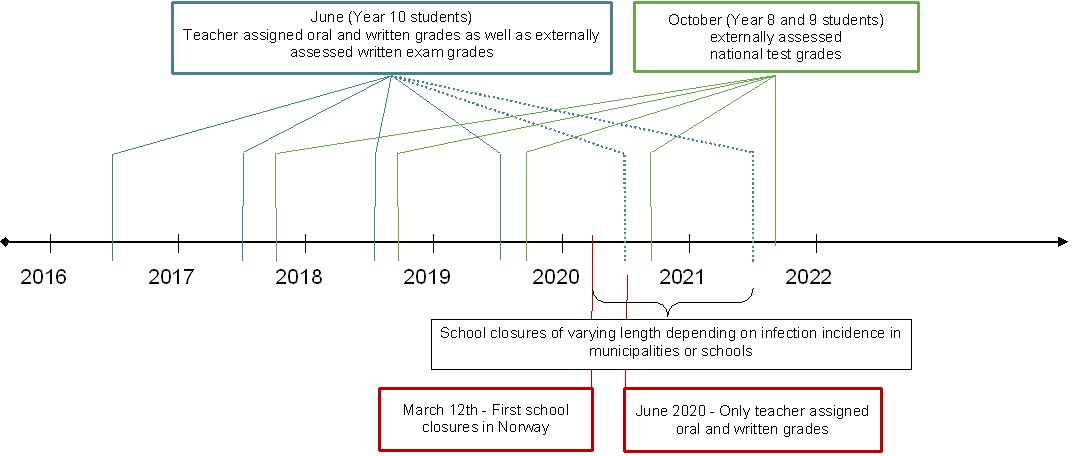
\includegraphics{timeline.jpg}
\end{figure}


\end{document}
